

\tikzset{every picture/.style={line width=0.75pt}} %set default line width to 0.75pt

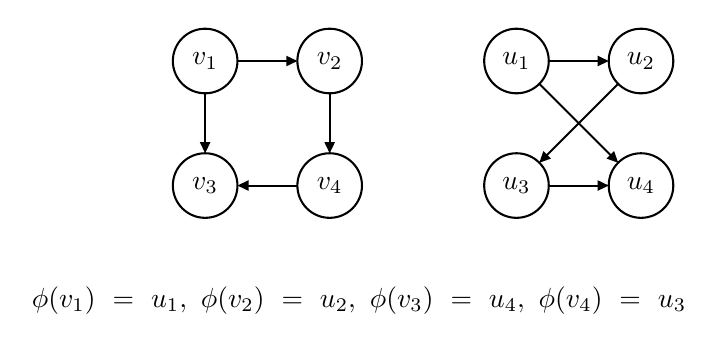
\begin{tikzpicture}[x=0.75pt,y=0.75pt,yscale=-1,xscale=1]
%uncomment if require: \path (0,300); %set diagram left start at 0, and has height of 300


% Text Node
\draw    (300, 20) circle [x radius= 15.56, y radius= 15.56]   ;
\draw (300,20) node   [align=left] {\begin{minipage}[lt]{13.600000000000001pt}\setlength\topsep{0pt}
\begin{center}
$\displaystyle v_{1}$
\end{center}

\end{minipage}};
% Text Node
\draw    (300, 80) circle [x radius= 15.56, y radius= 15.56]   ;
\draw (300,80) node   [align=left] {\begin{minipage}[lt]{13.600000000000001pt}\setlength\topsep{0pt}
\begin{center}
$\displaystyle v_{3}$
\end{center}

\end{minipage}};
% Text Node
\draw    (360, 80) circle [x radius= 15.56, y radius= 15.56]   ;
\draw (360,80) node   [align=left] {\begin{minipage}[lt]{13.600000000000001pt}\setlength\topsep{0pt}
\begin{center}
$\displaystyle v_{4}$
\end{center}

\end{minipage}};
% Text Node
\draw    (360, 20) circle [x radius= 15.56, y radius= 15.56]   ;
\draw (360,20) node   [align=left] {\begin{minipage}[lt]{13.600000000000001pt}\setlength\topsep{0pt}
\begin{center}
$\displaystyle v_{2}$
\end{center}

\end{minipage}};
% Text Node
\draw    (450, 20) circle [x radius= 15.56, y radius= 15.56]   ;
\draw (450,20) node   [align=left] {\begin{minipage}[lt]{13.600000000000001pt}\setlength\topsep{0pt}
\begin{center}
$\displaystyle u_{1}$
\end{center}

\end{minipage}};
% Text Node
\draw    (450, 80) circle [x radius= 15.56, y radius= 15.56]   ;
\draw (450,80) node   [align=left] {\begin{minipage}[lt]{13.600000000000001pt}\setlength\topsep{0pt}
\begin{center}
$\displaystyle u_{3}$
\end{center}

\end{minipage}};
% Text Node
\draw    (510, 80) circle [x radius= 15.56, y radius= 15.56]   ;
\draw (510,80) node   [align=left] {\begin{minipage}[lt]{13.600000000000001pt}\setlength\topsep{0pt}
\begin{center}
$\displaystyle u_{4}$
\end{center}

\end{minipage}};
% Text Node
\draw    (510, 20) circle [x radius= 15.56, y radius= 15.56]   ;
\draw (510,20) node   [align=left] {\begin{minipage}[lt]{13.600000000000001pt}\setlength\topsep{0pt}
\begin{center}
$\displaystyle u_{2}$
\end{center}

\end{minipage}};
% Text Node
\draw (215,127.4) node [anchor=north west][inner sep=0.75pt]    {$\phi ( v_{1}) \ =\ u_{1} ,\ \phi ( v_{2}) \ =\ u_{2} ,\ \phi ( v_{3}) \ =\ u_{4} ,\ \phi ( v_{4}) \ =\ u_{3}$};
% Connection
\draw    (315.56,20) -- (341.44,20) ;
\draw [shift={(344.44,20)}, rotate = 540] [fill={rgb, 255:red, 0; green, 0; blue, 0 }  ][line width=0.08]  [draw opacity=0] (5.36,-2.57) -- (0,0) -- (5.36,2.57) -- cycle    ;
% Connection
\draw    (360,35.56) -- (360,61.44) ;
\draw [shift={(360,64.44)}, rotate = 270] [fill={rgb, 255:red, 0; green, 0; blue, 0 }  ][line width=0.08]  [draw opacity=0] (5.36,-2.57) -- (0,0) -- (5.36,2.57) -- cycle    ;
% Connection
\draw    (344.44,80) -- (318.56,80) ;
\draw [shift={(315.56,80)}, rotate = 360] [fill={rgb, 255:red, 0; green, 0; blue, 0 }  ][line width=0.08]  [draw opacity=0] (5.36,-2.57) -- (0,0) -- (5.36,2.57) -- cycle    ;
% Connection
\draw    (300,35.56) -- (300,61.44) ;
\draw [shift={(300,64.44)}, rotate = 270] [fill={rgb, 255:red, 0; green, 0; blue, 0 }  ][line width=0.08]  [draw opacity=0] (5.36,-2.57) -- (0,0) -- (5.36,2.57) -- cycle    ;
% Connection
\draw    (465.56,20) -- (491.44,20) ;
\draw [shift={(494.44,20)}, rotate = 540] [fill={rgb, 255:red, 0; green, 0; blue, 0 }  ][line width=0.08]  [draw opacity=0] (5.36,-2.57) -- (0,0) -- (5.36,2.57) -- cycle    ;
% Connection
\draw    (465.56,80) -- (491.44,80) ;
\draw [shift={(494.44,80)}, rotate = 180] [fill={rgb, 255:red, 0; green, 0; blue, 0 }  ][line width=0.08]  [draw opacity=0] (5.36,-2.57) -- (0,0) -- (5.36,2.57) -- cycle    ;
% Connection
\draw    (499,31) -- (463.12,66.88) ;
\draw [shift={(461,69)}, rotate = 315] [fill={rgb, 255:red, 0; green, 0; blue, 0 }  ][line width=0.08]  [draw opacity=0] (5.36,-2.57) -- (0,0) -- (5.36,2.57) -- cycle    ;
% Connection
\draw    (461,31) -- (496.88,66.88) ;
\draw [shift={(499,69)}, rotate = 225] [fill={rgb, 255:red, 0; green, 0; blue, 0 }  ][line width=0.08]  [draw opacity=0] (5.36,-2.57) -- (0,0) -- (5.36,2.57) -- cycle    ;

\end{tikzpicture}